% R4 revised figures — English captions (A7). Terminology: "stepwise composition change" (was Schedule A),
% "client mobility" (was mobility-med), "late abrupt change" (was post-convergence abrupt).
% Numbers quoted in captions come from data/a4_f1_stats.csv (F1) and data/a1_segment_acc.csv (F7).

\begin{figure*}[t]\centering
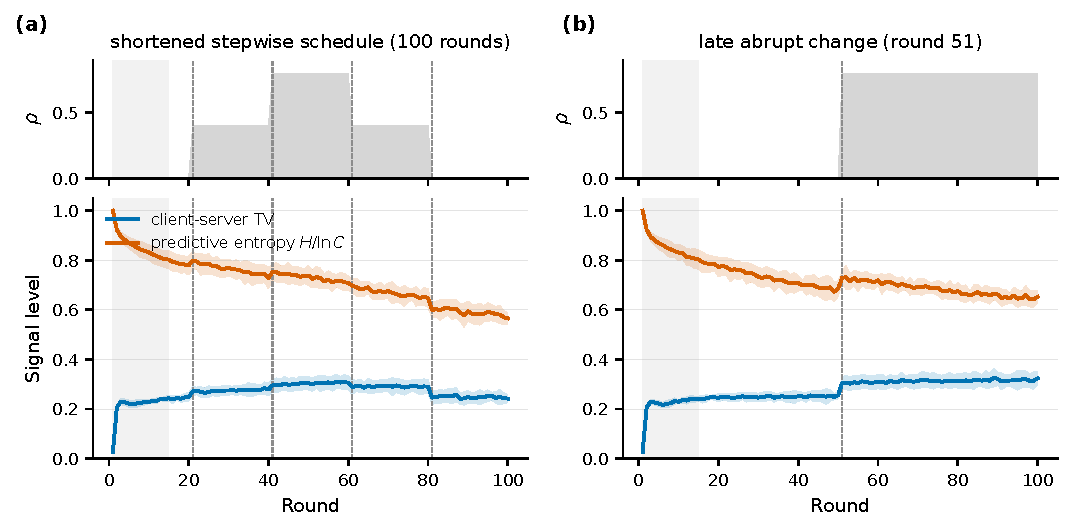
\includegraphics[width=\textwidth]{figures/fig01_signal_dynamics.pdf}
\caption{Signal dynamics on a fixed-weight model trajectory ($\lambda{=}0.4$, $\Lambda{=}0.5$; 3 seeds, bands = seed SD).
(a) Shortened stepwise schedule (100 rounds; $\rho$ changes at rounds 21/41/61/81). (b) Late abrupt change: $\rho$ steps
from 0 to 0.8 at round 51. Client--server TV (blue) rises with $\rho$ and returns with it. Normalized predictive entropy
$H/\ln C$ (orange) keeps decreasing as training continues: in (b) it rises by only $+0.037$ across the shift
(rounds 46--50 vs.\ 51--55) while it falls by $0.140$ from round 16 to the end, so the entropy level during the
shift stays below its pre-shift level; TV rises by $+0.055$ at the shift and ends $0.085$ above its round-16 level.
Warm-up rounds are shaded; dashed lines mark $\rho$ changes.}
\label{fig:signal_dynamics}
\end{figure*}

\begin{figure*}[t]\centering
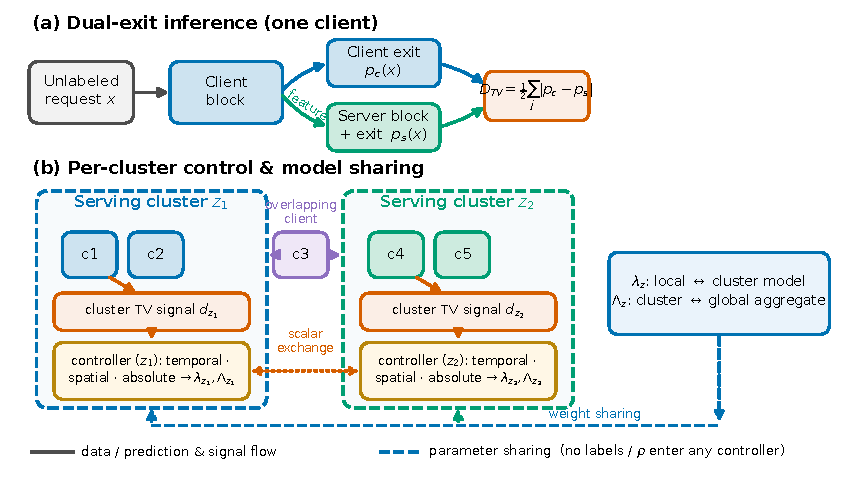
\includegraphics[width=0.9\textwidth]{figures/fig02_system_overview.pdf}
\caption{DriftGate overview. (a) Dual-exit inference: the client block feeds a client exit $p_c$ and, through the
server block, a server exit $p_s$; their total variation $D_{TV}$ is the unlabeled drift signal. (b) Control is
computed \emph{per serving cluster}: client TV values are averaged into a cluster signal, and each cluster's
controller turns it, via temporal/spatial/absolute views, into $\lambda_z$ (local$\leftrightarrow$cluster) and
$\Lambda_z$ (cluster$\leftrightarrow$global) mixing weights; neighbouring controllers exchange one scalar per
round. Solid = data/prediction and signal flow, dashed = parameter sharing. No labels or $\rho$ enter any
controller. Two clusters are shown as an example.}
\label{fig:overview}
\end{figure*}

\begin{figure*}[t]\centering
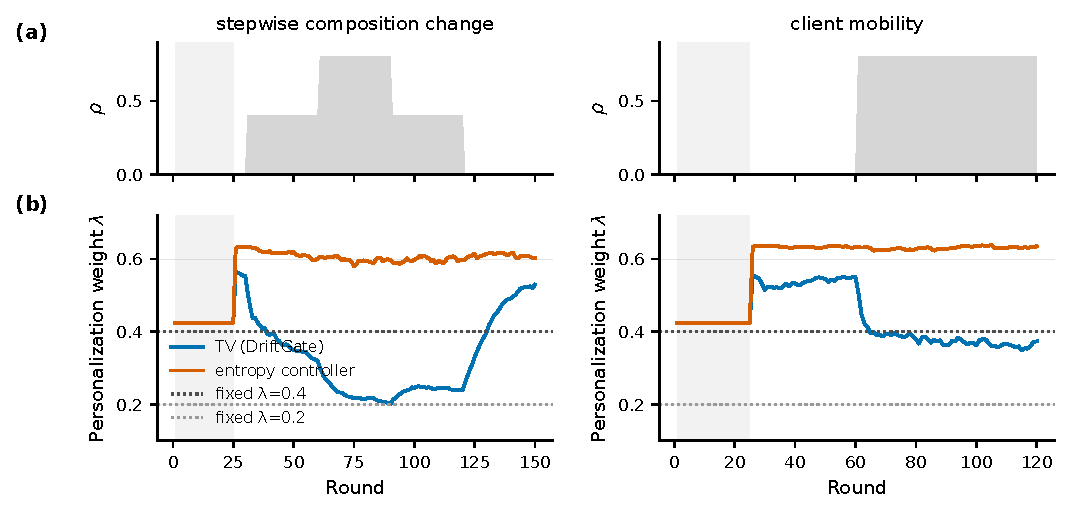
\includegraphics[width=\textwidth]{figures/fig03_lambda_adaptation.pdf}
\caption{Traffic change to $\lambda$ adaptation under the disjoint protocol. Left: stepwise composition change
(5 seeds); right: client mobility (3 seeds; $\rho$ steps to 0.8 at round 61 while cluster membership is re-evaluated
every 5 rounds). (a) $\rho$. (b) Per-cluster-averaged $\lambda$ for the TV controller and the entropy controller,
with fixed $\lambda{=}0.4$ and $0.2$ as dotted references. TV lowers $\lambda$ while $\rho$ is high and restores it
afterwards. The entropy controller, which in these runs used only the relative views, stays at
$\lambda\approx0.60$--$0.63$ after warm-up (the relative-view value at $q\approx0$). Rounds 1--25 (burn-in +
warm-up, shaded) use the midpoint $\lambda{=}0.425$.}
\label{fig:lambda_adaptation}
\end{figure*}

% F4: panel (b) is produced only after the B1 view-removal runs finish (data/b1_view_removal.csv).
\begin{figure*}[t]\centering
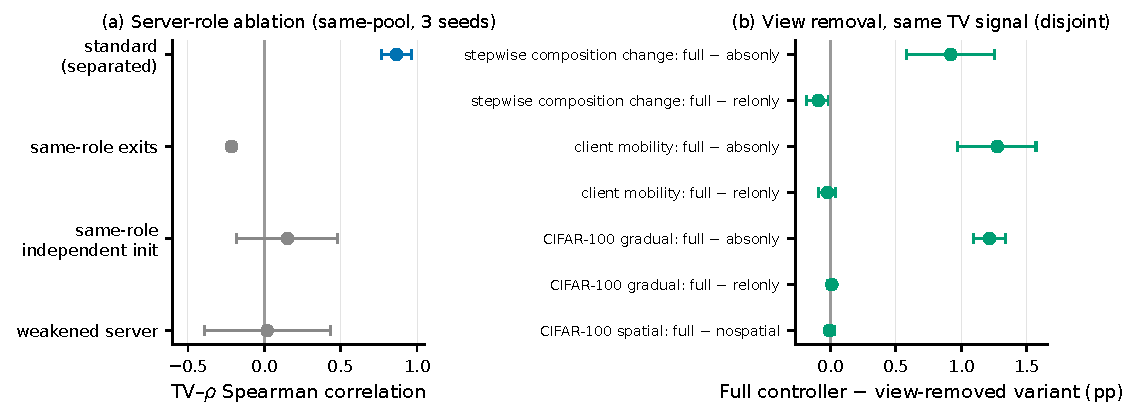
\includegraphics[width=\textwidth]{figures/fig04_mechanism_and_views.pdf}
\caption{(a) Server-role ablation: TV--$\rho$ Spearman correlation across role perturbations (same-pool, 3 seeds;
mean$\pm$SD). Separating the exits' roles is necessary for TV to track $\rho$. (b) View removal with the same TV
signal (disjoint): full controller minus the absolute-only, relative-only, or no-spatial variant (paired, 95\% CI).}
\label{fig:mechanism}
\end{figure*}

\begin{figure}[t]\centering
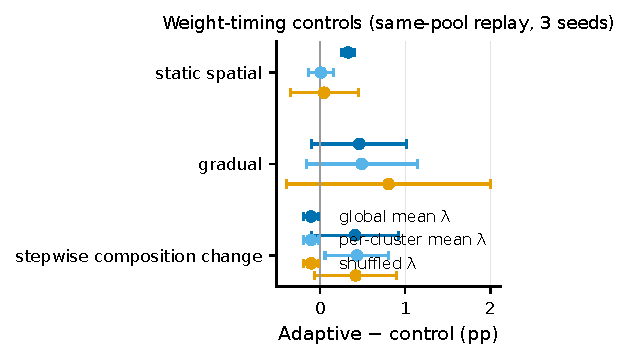
\includegraphics[width=\columnwidth]{figures/fig05_timing_controls.pdf}
\caption{Weight-timing controls: adaptive minus mean-matched and shuffled $\lambda$ policies (same-pool replay that
retrains with the altered weight order; 3 seeds, 95\% CI). On the static spatial setting the gain comes from good
per-cluster means, not from timing. (The adaptive-$\Lambda$ contribution is reported in the tables: $-0.07$ and
$+0.07$ pp with CIs including zero.)}
\label{fig:timing}
\end{figure}

\begin{figure}[t]\centering
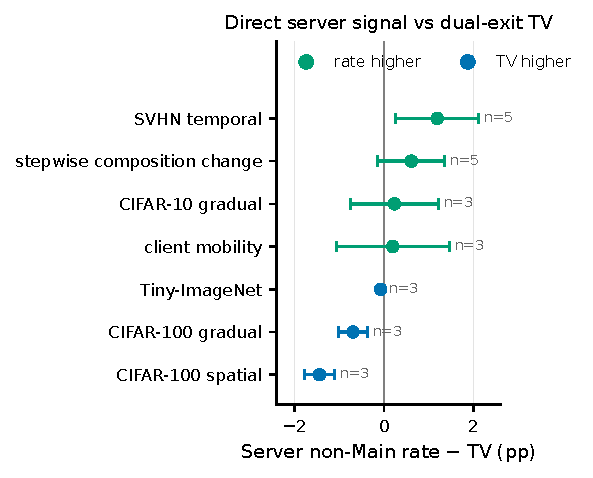
\includegraphics[width=\columnwidth]{figures/fig06_server_signal_comparison.pdf}
\caption{Direct server-only signal vs.\ dual-exit TV across seven settings (disjoint, paired; 95\% CI). The server
non-Main prediction rate matches or beats TV where the class count is small and the drift is real (SVHN, CIFAR-10)
but is weaker on many-class CIFAR-100. Green = rate higher, blue = TV higher.}
\label{fig:server_signal}
\end{figure}

\begin{figure*}[t]\centering
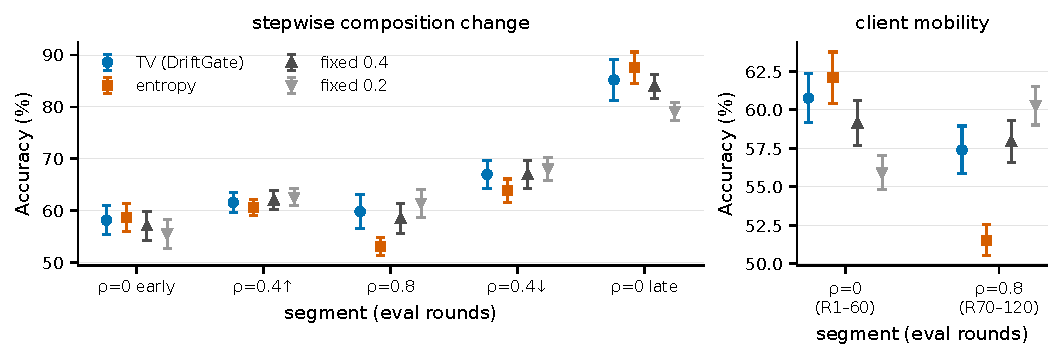
\includegraphics[width=\textwidth]{figures/fig07_segment_accuracy.pdf}
\caption{Segment accuracy (mean over the evaluation rounds in each segment; error bars = seed SD; disjoint
protocol). Left: stepwise composition change (5 seeds; segments $\rho{=}0$ early, $\rho{=}0.4$ rising, $\rho{=}0.8$,
$\rho{=}0.4$ falling, $\rho{=}0$ late). Right: client mobility (3 seeds; $\rho{=}0$ rounds 1--60 and $\rho{=}0.8$
rounds 70--120). TV's advantage over fixed $\lambda{=}0.4$ under mobility comes from the $\rho{=}0$ segment
($+1.63$ pp), not from the $\rho{=}0.8$ segment ($-0.54$ pp); fixed $\lambda{=}0.2$ is the best policy in the
sustained $\rho{=}0.8$ segments of both settings.}
\label{fig:segments}
\end{figure*}
